\documentclass[a4paper,12pt]{article}

%%%%%%%%%%%%%%%%%%%%
% Packages
%%%%%%%%%%%%%%%%%%%%
\usepackage[english]{babel}
\usepackage[T1]{fontenc}
\usepackage{amsmath}
\usepackage{cmbright}  % European Computer Modern Bright font
\usepackage{graphicx}  % Required for inserting images
\usepackage[margin=0cm]{geometry}
\usepackage{nopageno}
\usepackage{xcolor}
\usepackage{tikz}
\usepackage{tikzpagenodes}
\usepackage{fancyhdr}
\usepackage{enumitem}
\usepackage{booktabs}
\usepackage[defaultlines=2,all]{nowidow}
\usepackage[skip=0em]{parskip}
\usepackage{multicol}
\usepackage[hidelinks]{hyperref}

\usetikzlibrary{backgrounds}  % allows framed option for tikzpicture

%%%%%%%%%%%%%%%%%%%%
% Colours
%%%%%%%%%%%%%%%%%%%%
%\definecolor{accentcolour}{HTML}{359EBF}  % electric blue
\definecolor{accentcolour}{HTML}{e3a619}  % gold

\definecolor{subduedcolour}{HTML}{999999}

%%%%%%%%%%%%%%%%%%%%
% Tikz
%%%%%%%%%%%%%%%%%%%%

\tikzset{
    header node/.style={accentcolour, yshift=-1em, text depth=0.4em},
    header line/.style={line width=0.7mm, accentcolour, yshift=0.2},
    body node/.style={text width=12.5cm, align=justify},
    skills node/.style={black!75, yshift=-0em}
}

%%%%%%%%%%%%%%%%%%%%
% Headers & footers
%%%%%%%%%%%%%%%%%%%%
\fancyhf{}
\renewcommand{\headrulewidth}{0pt}
\fancyfoot[R]{\small \textcolor{subduedcolour}{\lastupdated}}
\pagestyle{fancy}

%%%%%%%%%%%%%%%%%%%%
% Other Layout Details
%%%%%%%%%%%%%%%%%%%%
\renewcommand{\arraystretch}{1.4}

\input{template/macros}

\begin{document}

    \begin{tikzpicture}[remember picture,overlay,anchor=north west,align=left]

        % Sidebar
        \node[fill=accentcolour, minimum width=\sidebarwidth, minimum height=\paperheight] at (current page.north west) (sidebar) {};

        % Anchors
        \node[] at (0.6em, 0) (sidebarleft) {};
        \node[] at (\sidebarwidth + 1.2em, 0) (bodyleft) {};
        \node[] at (\paperwidth - 1.5cm, 0) (bodyright) {};

        % Photo
        \begin{scope}
            \clip (0.5*\sidebarwidth,-0.5*\sidebarwidth+1em) circle (0.5*\picturewidth);
            \node[anchor=center, xshift=0.5*\sidebarwidth, yshift=-0.5*\sidebarwidth] at (current page.north west) (photo) {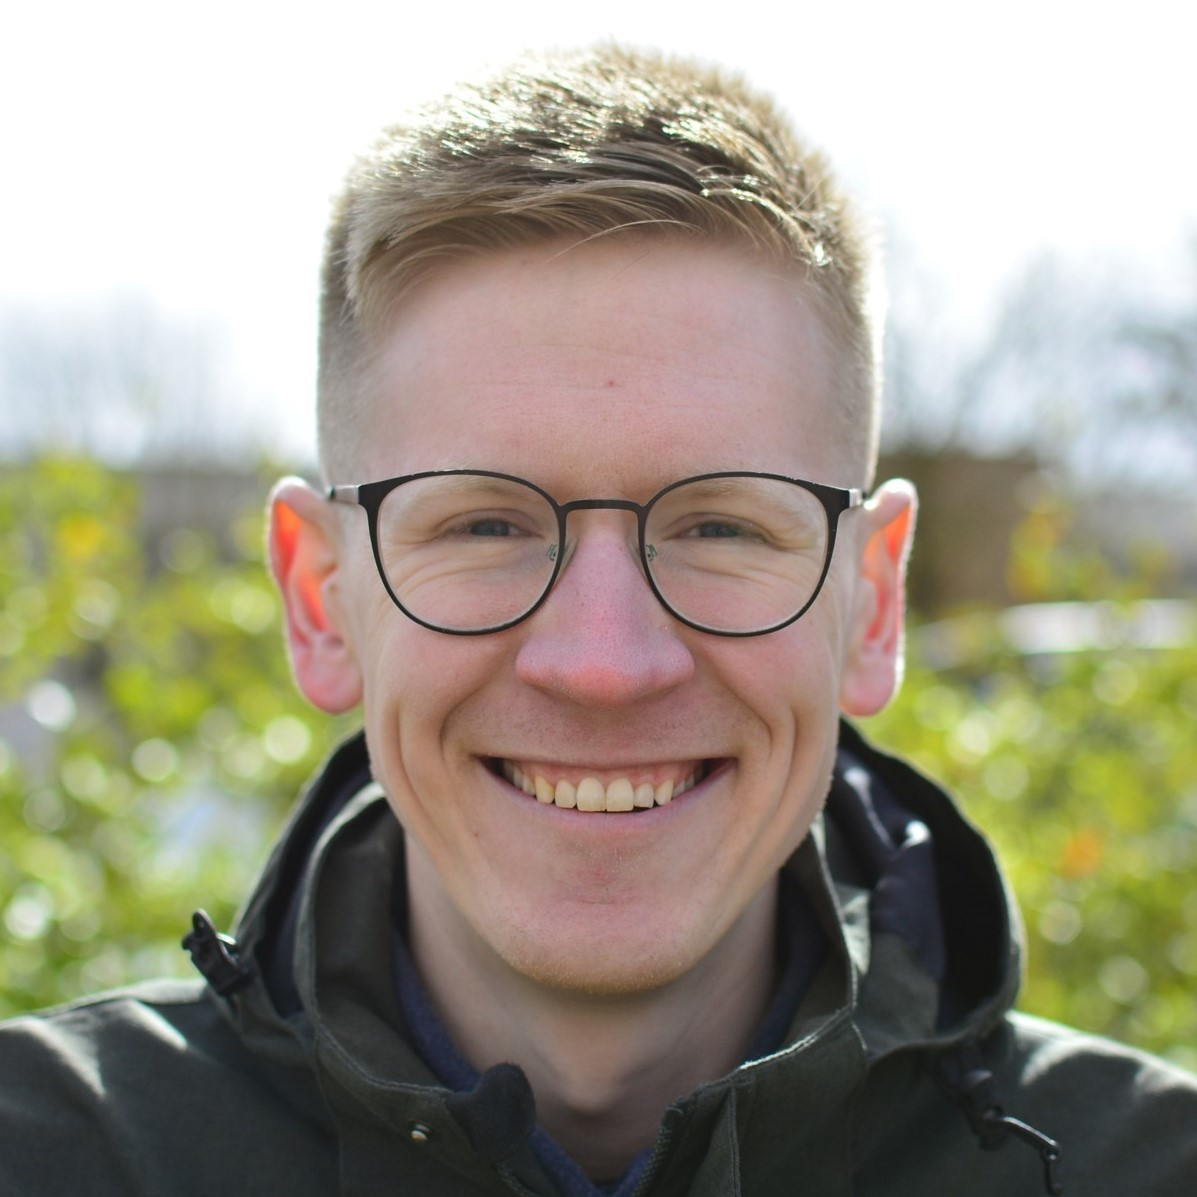
\includegraphics[width=\picturewidth]{profile_sq.jpg}};
            \draw[white, line width=1.5mm] (0.5*\sidebarwidth,-0.5*\sidebarwidth+1em) circle (0.5*\picturewidth);
        \end{scope}

        %%%%%%%%%%%%%%%%%%%%%%%%%%%%
        % Sidebar content
        %%%%%%%%%%%%%%%%%%%%%%%%%%%%

        % Technical skills
        \node[skills node, yshift=-1.5em] at (sidebarleft |- photo.south west) (techskills) {
            \textbf{Technical Skills} \\[0.4em]
            \mybullet{} Algorithm design \\[\listspacing]
            \mybullet{} Software development \\[\listspacing]
            %\mybullet{} Scripting \\[\listspacing]
            \mybullet{} Data structures \\[\listspacing]
            %\mybullet{} OOP \\[\listspacing]
            \mybullet{} Data analytics \\[\listspacing]
            \mybullet{} Predictive modelling \\[\listspacing]
            \mybullet{} Natural language analysis \\[\listspacing]
            \mybullet{} REST API development \\[\listspacing]
            \mybullet{} Software testing, TDD \\[\listspacing]
        };
        % Software languages
        \node[skills node] at (sidebarleft |- techskills.south west) (softwarelanguages) {
            \textbf{Software languages} \\[0.4em]
            \mybullet{} Python (advanced) \\[\listspacing]
            \mybullet{} C/C++ (intermediate) \\[\listspacing]
        };
        % Tools
        \node[skills node] at (sidebarleft |- softwarelanguages.south west) (tools) {
            \textbf{Tools/packages} \\[0.4em]
            \mybullet{} VS Code \\[\listspacing]
            \mybullet{} Git \\[\listspacing]
            \mybullet{} SQL \\[\listspacing]
            \mybullet{} Jupyter \\[\listspacing]
            %\mybullet{} MySQL \\[\listspacing]
            \mybullet{} Postman \\[\listspacing]
        };
        % Soft skills
        \node[skills node] at (sidebarleft |- tools.south west) (softskills) {
            \textbf{Soft Skills} \\[0.4em]
            \mybullet{} Problem solving \\[\listspacing]
            \mybullet{} Research \\[\listspacing]
            \mybullet{} Public speaking \\[\listspacing]
            \mybullet{} Collaboration \\[\listspacing]
            \mybullet{} Documentation \\[\listspacing]
        };
        % Languages
        \node[skills node] at (sidebarleft |- softskills.south west) (softwarelanguages) {
            \textbf{Languages} \\[0.4em]
            \mybullet{} English (native) \\[\listspacing]
            \mybullet{} Danish (fluent) \\[\listspacing]
        };

        %%%%%%%%%%%%%%%%%%%%%%%%%%%%
        % Body content
        %%%%%%%%%%%%%%%%%%%%%%%%%%%%

        % Headline
        \node[anchor=west, align=left] at (photo.east -| bodyleft) (headline) {
            \Huge \textcolor{accentcolour}{\textbf{\name{}}} \\[0.5em]
            Researcher | Data Scientist | Software Developer \\
            % Dedicated researcher, curious about data and enthusiastic about software \\
        };
        \node[xshift=-0.5em, yshift=1.0em] at (headline.south west) (contact) {\input{template/header}};

        % Profile
        \node[header node] at (contact.south -| bodyleft) (profile) {\Large\textbf{Profile}};
        \draw[header line] (profile.east)+(0.5em,0) -- (profile -| bodyright)+(-2cm,0);
        \node[body node, yshift=0.4em] at (profile.south west) (profilebody) {
            I am a professional and dedicated engineer with strong competencies in software development, deep technical understanding in data compression and analytics and a drive to satisfy customers.
%            He holds BSc (2016) and Masters (2018) degrees in electronic engineering from The University of Western Australia, together with a PhD from Aarhus University (2024).
            My current research as a postdoc at Aarhus University focuses on data compression, big data analytics and sensor calibration, especially within the context of IoT systems.
            I am currently looking for an opportunity to move back to industry where I can more directly support customer outcomes and hope to join a high performing and innovative team where I can grow rapidly.
        };


        % Experience
        \node[header node] at (profilebody.south -| bodyleft) (experience) {\Large\textbf{Experience}};
        \draw[header line] (experience.east)+(0.5em,0) -- (experience -| bodyright)+(-2cm,0);
        \node[body node] at (experience.south west) (e1) {
            \textbf{Postdoctoral Fellow} \hfill {\footnotesize\color{subduedcolour}Nov 2023--Present} \\[0.2em]
            Department of Electronic \& Computer Engineering, Aarhus University
            \begin{itemize}[itemsep=-1pt,topsep=0.4em]
                \item Investigating the application of state-of-the-art data compression and analytics research to practical and commercial contexts.
                \item Developing robust techniques for optimising the quality of sensor data using limited calibration information.
                \item Leading collaborations with Aarhus University Department of Biology and Villanova University.
            \end{itemize}
        };
        \node[body node] at (e1.south west) (e2) {
            \textbf{PhD Fellow} \hfill {\footnotesize\color{subduedcolour}Nov 2020--Nov 2023} \\[0.2em]
            Department of Electronic \& Computer Engineering, Aarhus University
            \begin{itemize}[itemsep=-1pt,topsep=0.4em]
                \item Investigating the joint optimisation of lossless data compression and data analytics for IoT applications.
                \item Developing algorithms and software for high-efficiency data analytics and querying, prioritising storage, accuracy and latency.
                \item Optimising federated learning communication efficiency using novel compression techniques in collaboration with Professor Tara Javidi of UCSD.
            \end{itemize}
        };
        \node[body node] at (e2.south west) (e3) {
            \textbf{Data Scientist/Consultant} \hfill {\footnotesize\color{subduedcolour}Feb 2018--Jul 2020} \\[0.2em]
            IBM Australia
            \begin{itemize}[itemsep=-1pt,topsep=0.4em]
                \item Leading a team of developers in building a decision-support web application for a large mining company.
                \item Establishing data science processes and software for predictive maintenance at a state water utility.
                \item Developing natural language models to help clients leverage non-structured data in business decision making.
            \end{itemize}
        };


    \end{tikzpicture}

    \pagebreak

    %%%%%%%%%%%%%%%%%%%%%%%%%%%%%%%%%%%%
    % Page 2
    %%%%%%%%%%%%%%%%%%%%%%%%%%%%%%%%%%%%

    \begin{tikzpicture}[remember picture,overlay,anchor=north west,align=left]

            % Sidebar
            \node[fill=accentcolour, minimum width=\sidebarwidth, minimum height=\paperheight] at (current page.north west) (sidebar) {};

            % Anchors
            \node[] at (0.6em, 0) (sidebarleft) {};
            \node[] at (\sidebarwidth + 1.2em, -1.5em) (bodyleft) {};
            \node[] at (\paperwidth - 1.5cm, -1.5em) (bodyright) {};

            %%%%%%%%%%%%%%%%%%%%%%%%%%%%
            % Sidebar content
            %%%%%%%%%%%%%%%%%%%%%%%%%%%%

            % Publications
            \node[skills node, text width=5.4cm, anchor=north west, yshift=-2.5em] at (sidebarleft) (publications) {
                \textbf{Publications} \\[0.4em]
                First author:
                \begin{itemize}[itemsep=1pt,topsep=0.3em,leftmargin=*]
                    \item PairwiseHist: Fast, Accurate, and Space-Efficient Approximate Query Processing with Data Compression, \textit{VLDB}, 2024.
                    \item GreedyGD: Enhanced Generalized Deduplication compression for IoT applications, \textit{IEEE TII}, 2024.
                    \item GLEAN: Generalized Deduplication enabled approximate edge analytics, \textit{IEEE IoT Journal}, 2022.
                    \item Direct analytics of generalized deduplication compressed IoT data, \textit{IEEE GLOBECOM}, 2021.
                    \item A Low-Cost Hardware-in-the-Loop Agent-Based Simulation Testbed for Autonomous Vehicles, \textit{IEEE/ASME AIM}, 2018.
                \end{itemize}
                \vspace{0.5em}
                Co-author:
                \begin{itemize}[itemsep=1pt,topsep=0.3em,leftmargin=*]
                    \item Reconfigurable magnetic domain wall pinning using vortex-generated magnetic fields, \textit{Applied Physics Letters}, 2017.
                \end{itemize}
            };


            %%%%%%%%%%%%%%%%%%%%%%%%%%%%
            % Body content
            %%%%%%%%%%%%%%%%%%%%%%%%%%%%

            % Education
            \node[header node] at (bodyleft) (education) {\Large\textbf{Education}};
            \draw[header line] (education.east)+(0.5em,0) -- (education -| bodyright)+(-2cm,0);
            \node[body node] at (education.south west) (e1) {
                \textbf{Master of Professional Engineering} \hfill {\footnotesize\color{subduedcolour}Feb 2016--Dec 2017} \\[0.2em]
                The University of Western Australia
                \begin{itemize}[itemsep=-2pt,topsep=0.4em]
                    \item Specialisation: Electrical \& Electronic Engineering.
                    \item Thesis: Autonomous vehicle testbed computer vision system.
                    \item Highest average grade in my cohort of 298 students.
                    %\item Five prizes for top marks in individual courses.
                \end{itemize}
            };
            \node[body node] at (e1.south west) (e2) {
                \textbf{Bachelor of Science} \hfill {\footnotesize\color{subduedcolour}Feb 2013--Dec 2015} \\[0.2em]
                The University of Western Australia
                \begin{itemize}[itemsep=-1pt,topsep=0.4em]
                    \item Majors: Electronic Engineering \& Management.
                    \item Highest average grade in my cohort.
                    \item Delivered the valedictory address at my graduation ceremony.
                    %\item Rio Tinto Undergraduate Scholarship in Geology and/or Engineering Science \textcolor{subduedcolour}{(for academic achievement).}
                    %\item Tesla Medal in Electronic Materials and Devices \textcolor{subduedcolour}{(highest mark in my cohort)}.
                \end{itemize}
            };

        % Awards & accomplishments
        \node[header node] at (e2.south west) (awards) {\Large\textbf{Awards}};
        \draw[header line] (awards.east)+(0.5em,0) -- (awards -| bodyright)+(-2cm,0);
        \node[body node] at (awards.south west) (awardsbody) {
            \begin{tabular}{lp{0.87\textwidth}}
                \textbf{2024} & \textbf{Thomas B. Triges Fond.} Awarded to support traveling to present my research at a prestigious international conference. [15,000 kr] \\
                \textbf{2023} & \textbf{EliteForsk-rejsestipendium.} Awarded by The Danish Ministry of Higher Education and Science to 20 PhD students annually to support international research visits. [200,000 kr] \\
            \end{tabular}
        };

        % Other experience
        \node[header node] at (awardsbody.south west) (otherexperience) {\Large\textbf{Other Experience}};
        \draw[header line] (otherexperience.east)+(0.5em,0) -- (otherexperience -| bodyright)+(-2cm,0);
        \node[body node] at (otherexperience.south west) (e1) {
            \textbf{Student Rail Engineer} \hfill {\footnotesize\color{subduedcolour}Dec 2016--Feb 2017} \\[0.2em]
            Public Transport Authority, Western Australia
            %\begin{itemize}[itemsep=-2pt,topsep=0.4em]
            %    \item Assisted with documentation management, asset reliability assessments and design verifications.
            %\end{itemize}
        };
        \node[body node] at (e1.south west) (e2) {
            \textbf{Tutor/Class Facilitator} \hfill {\footnotesize\color{subduedcolour}Feb 2016--Nov 2017} \\[0.2em]
            The University of Western Australia
            %\begin{itemize}[itemsep=-1pt,topsep=0.4em]
            %    \item Facilitated classes of 10--40 students in statistics, project management and semiconductor materials.
            %\end{itemize}
        };
        \node[body node] at (e2.south west) (e3) {
            \textbf{Research Intern} \hfill {\footnotesize\color{subduedcolour}Dec 2015--Feb 2016} \\[0.2em]
            Pawsey Supercomputing Centre
            %\begin{itemize}[itemsep=-1pt,topsep=0.4em]
            %    \item Investigating novel magneto-electronic devices using simulations run on Pawsey's supercomputers.
            %\end{itemize}
        };

        \node[header node] at (e3.south west) (aboutme) {\Large\textbf{About Me}};
        \draw[header line] (aboutme.east)+(0.5em,0) -- (aboutme -| bodyright)+(-2cm,0);
        \node[body node, yshift=0.4em] at (aboutme.south west) (aboutmebody) {
            I am married to Rebecca and together we have a 9-month-old son and a 40-year-old house in Aarhus Vest, which we are gradually renovating.
            Family, church, running and home improvement projects fill most of my spare time.
            In between, I love reading, photography and board games---especially long, strategic ones.
        };




    \end{tikzpicture}



%%\section{Accomplishments}
%%
%%\noindent
%%\begin{tabular}{lp{0.87\textwidth}}
%%    \textbf{2023} & EliteForsk-rejsestipendium. \textcolor{subduedcolour}{The Danish Ministry of Higher Education and Science awards up to 20 stipends each year of 200,000 DKK to support PhD students undertaking international research visits. Candidates must be selected and proposed by their institute.} \\
%%
%%    \textbf{2022} & Passed Prøve i Dansk 3 (PD3) with top marks across all disciplines. \textcolor{subduedcolour}{This is the highest level standard Danish exam and a pre-requisite for certain permanent visas and citizenship.}\\
%%
%%    \textbf{2019} & Industrial Products Insights and Solutions (Bronze). \textcolor{subduedcolour}{Awarded by IBM based on experience and contributions to clients within industrial sectors.} \\
%%
%%    \textbf{2016} & Institution of Engineering and Technology Prize in Communication Systems. \textcolor{subduedcolour}{Awarded to the student who achieved the highest course grade. AU\$300 and one year membership.} \\
%%
%%    & MRX Technologies Prize in Control Engineering. \textcolor{subduedcolour}{Awarded to the student who achieved the highest course grade. AU\$1.000.} \\
%%
%%    & MRX Technologies Prize in Digital and Embedded Systems. \textcolor{subduedcolour}{Awarded to the student who achieved the highest course grade. AU\$1.000.} \\
%%
%%    & Monadelphous Prize in Project Management and Engineering Practice,. \textcolor{subduedcolour}{Awarded to the student who achieved the highest course grade. AU\$1.500.} \\
%%
%%    & Programmed Professionals Prize in Circuits and Electronic Systems. \textcolor{subduedcolour}{Awarded to the student who achieved the highest course grade. AU\$2.000.} \\
%%
%%    \textbf{2015} & Rio Tinto Undergraduate Scholarship in Geology and/or Engineering Science for academic achievement. \textcolor{subduedcolour}{Awarded to two students annually based on academic performance. AU\$6.000 and invitation to two masterclass workshops.} \\
%%
%%    & Selected to give the valedictory address at my bachelor graduation ceremony. \\
%%
%%    & Tesla Medal in Electronic Materials and Devices. \textcolor{subduedcolour}{Awarded to the student who achieved the highest course grade. % ENSC3014 Electronic Materials and Devices.
%%    Cash prize and a physical medal.} \\
%%
%%    \textbf{2014} & John \& Robin de Laeter Scholarshop. \textcolor{subduedcolour}{Awarded for restoring science education exhibits at the Gravidt Discovery Centre museum, Gingin, Western Australia.}
%%\end{tabular}



\end{document}

